\documentclass[english,11pt]{l4proj}
\usepackage[T1]{fontenc}
\usepackage[utf8]{inputenc}
\usepackage{graphicx}
\usepackage{geometry}
\usepackage{caption}
\usepackage{babel}
\usepackage{amsmath}
\usepackage{verbatim}
\usepackage{hyperref}
\usepackage{algpseudocode}
\usepackage{algorithm}
\usepackage{subcaption}
\usepackage{appendix}

\renewcommand*\thesection{\arabic{section}}

\begin{document}

\title{Paxos on many-core platforms}
\author{Motiejus Jakštys}
\date{21 March 2013}

\maketitle

\begin{abstract}

Current many-core chips look alike to many-node clusters. Many-core systems,
like many-machine systems, need redundancy in order to be robust.
Synchronization techniques used in cluster computing start applying in smaller
scale, for many-core chips. In this project we research ability of an
application of distributed synchronization, state machine replication, on a
many-core chip.

The work looks at many-core programming approaches, and, as a use case,
implements and test Classic Paxos in Erlang on a 64-core network-on-chip
TILEPro64.

\end{abstract}

\tableofcontents
\pagebreak

\section{Introduction}

\subsection{Report outline}

Section~\ref{sec:many-core} presents how computing in many-core systems changed
recently. Section~\ref{sec:tilera} shows why Tilera64 was chosen as development
platform. Section~\ref{sec:paxos-family} presents what consensus algorithms are.
Section~\ref{sec:erlang-why} explains why Erlang was chosen for this
application, and section~\ref{sec:erlang-eval} evaluates Erlang suitability for
many-core platforms.

Section~\ref{sec:paxos-api} shows the API and architecture of classic Paxos.
Section~\ref{sec:conclusion} presents conclusions and future work.

\subsection{Changes in Moore's law}
\label{sec:many-core}

During the last decade Moore's law had changed the rules of machine performance.
Clock speeds used to double every three years. However, recently frequency
limits have been reached due to minimum possible sizes of the chips. On the
other hand, given clock speed limits, number of cores on a chip started
increasing rapidly. 8-core CPUs are now very common in commodity desktop
systems, and servers with 24 cores are more and more widely deployed.

In order to go further improving the performance, increasing the frequency does
not pay off; other approach is needed. According to inverse Pollack's
rule\cite{pollack}, highest computational bandwidth will be achieved by
parallelizing the work on many small cores\cite{1kcorechips}.

Borkar et. al. goes into more detail about this\cite{future-microprocessors}:

\begin{quote}

    To explore this concept further, consider three systems on a chip
    comprising 1: 12 large (60MT) cores, 2: 48 medium (15MT) cores, and 3: 144
    small (5MT) cores, all of them with the same amount of total cache, and all
    of them in the same power envelope. Figure~\ref{fig:core_size_performance}
    compares their relative performance.

    Small core is 12 times smaller than the large core, but its performance is
    only about a third of the large core. Total throughput of the small core
    system (TPT), however, is much higher than the large core system. If you
    parallelize one application for a 12 large core system and a 144 small core
    system then the small core system performs poorly, as expected from Amdahl’s
    Law\cite{amdahls-law}. Notice that as the number of applications increase,
    total system performance of medium and small core systems increase.
    Therefore, to harvest the performance of a many-core system, we cannot just
    depend on parallelizing a single application, but must utilize task level
    and application level parallelism.

\end{quote}

\begin{figure}[h]
    \centering
    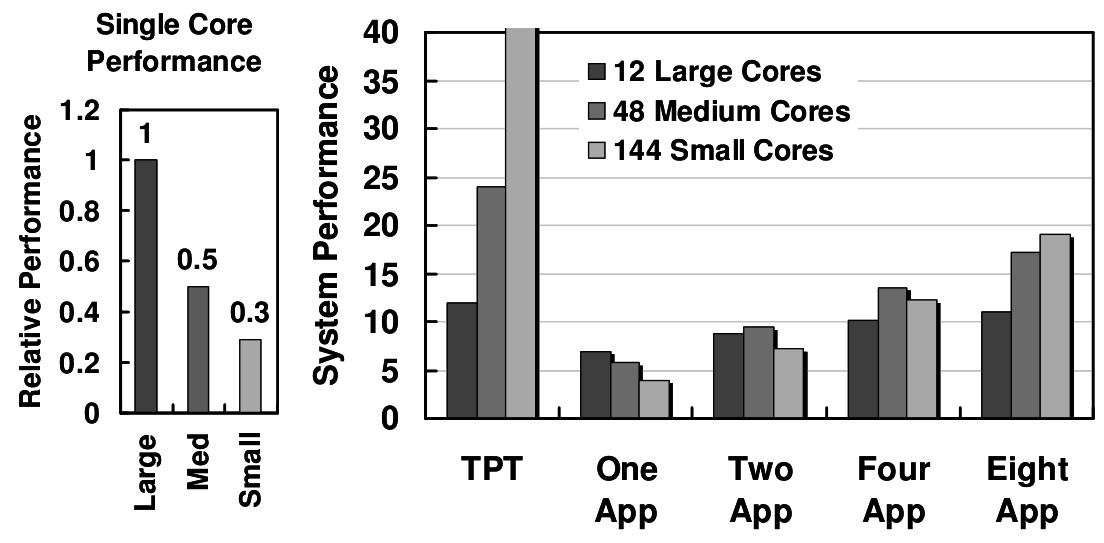
\includegraphics[width=0.5\textwidth]{images/pollack.png}
    \caption{Performance of Large, Medium and Small
    Cores\cite{future-microprocessors}}
    \label{fig:core_size_performance}
\end{figure}

However, application performance suffers from its serial factor, which is
formally described by Amdahl's law:

$$
\text{Parallel speedup} =
\frac{1}{\text{Serial \%} + (1 - \text{Serial \%}) / N}
$$

If serial percentage is large, then parallel speedup saturates with small number
of cores. Figure~\ref{fig:amdahl} illustrates the impact of serial
percentage of code on parallel speedup.

\begin{figure}[h]
    \centering
    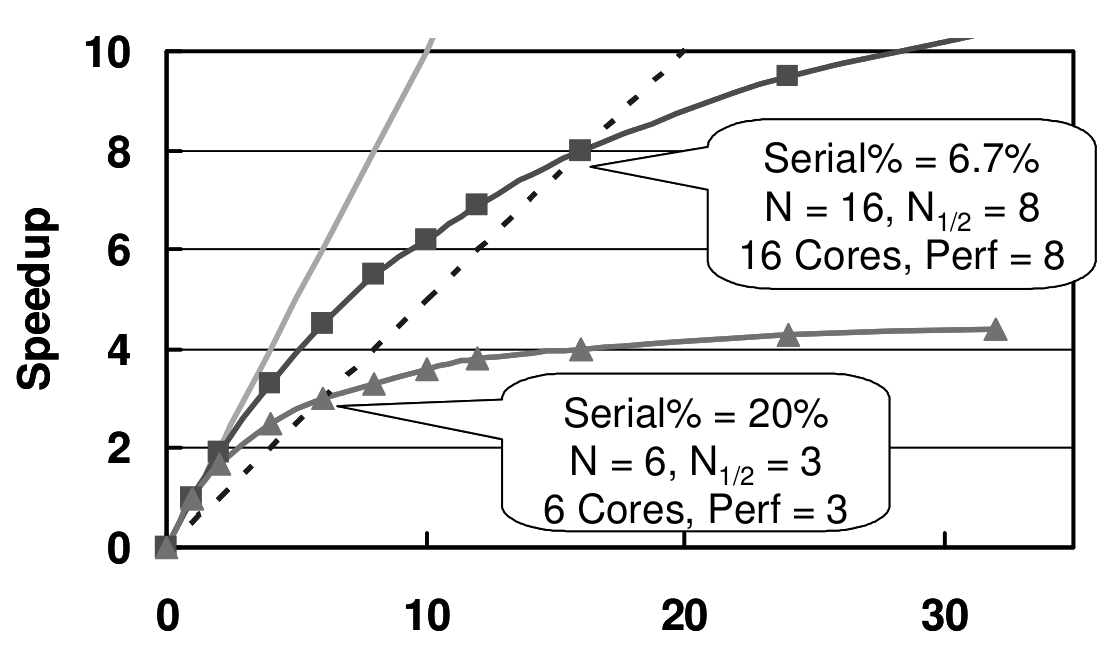
\includegraphics[width=0.5\textwidth]{images/amdahl.png}
    \caption{Amdahl's Law limits parallel speedup\cite{future-microprocessors}}
    \label{fig:amdahl}
\end{figure}

This is where the future of microprocessors is heading to: having more less
powerful cores to do the work\cite{future-microprocessors}, and programming
languages and tools are developed to make parallel programming easier, i.e. to
reduce the serial component.

The conclusions are that it is very important to reduce serial part of the
program. In practice, it is complicated to get it right. We will come back to
this further in the report.

\section{Trends in many-core architectures}
\label{sec:manycore-trends}

In order to solve performance improvement problems described in
section~\ref{sec:many-core}, during recent years there has been much movement in
many-core hardware development\footnote{Intel Tera:
\url{http://www.intel.com/pressroom/kits/teraflops/}} \footnote{Adapteva and
Parallella: \url{http://www.adapteva.com/}} \footnote{Tilera:
\url{http://www.tilera.com/}}. We will look at two similar network-on-chip
approaches.

\subsection{TILEPro64 by Tilera}
\label{sec:tilera}

\begin{figure}
    \centering
    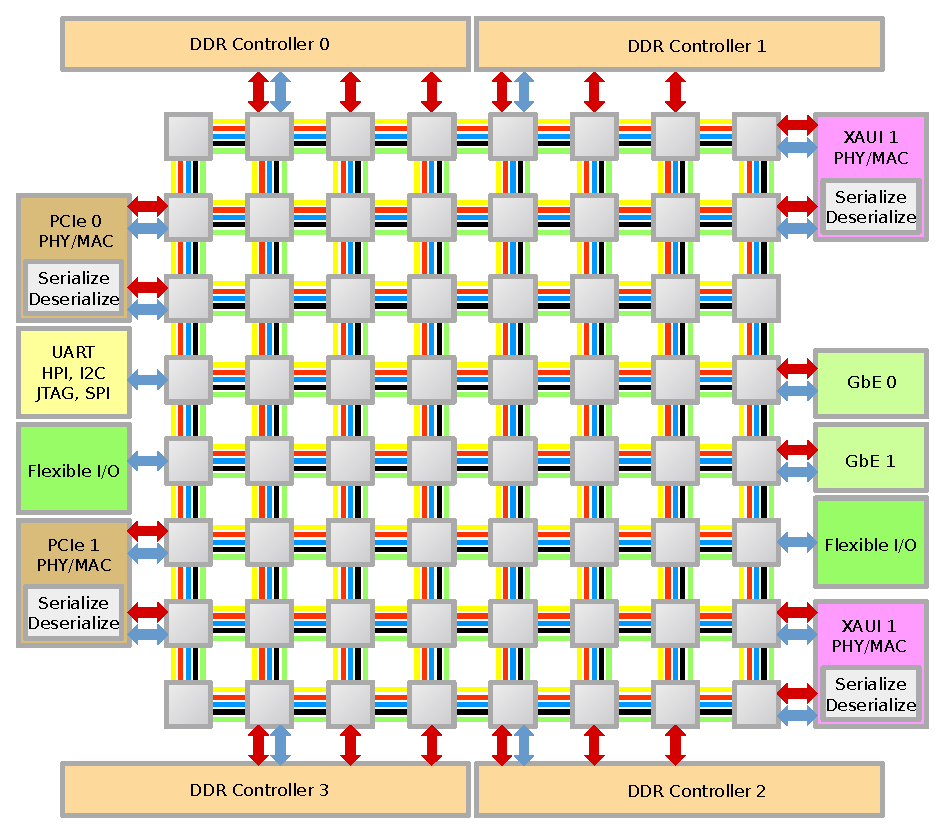
\includegraphics[width=0.5\textwidth]{images/tile64.pdf}
    \caption{TILEPro64 processor network block diagram\cite{tilepro64-diagram}}
    \label{fig:tile64}
\end{figure}

Figure~\ref{fig:tile64} is the block diagram of TILEPro64 processor. It consists
of a mesh network of 64 {\em tiles}, where each {\em tile} houses a general
purpose processor, cache, and a non-blocking router, which the tile uses to
communicate with the other tiles on the processor.

There is high-speed, low-latency packet-switched network between the cores for a
few purposes. Most interesting are two: shared L3 cache and User Dynamic
Network, UDN.

\subsubsection{Shared L3 cache}
\begin{figure}
    \centering
    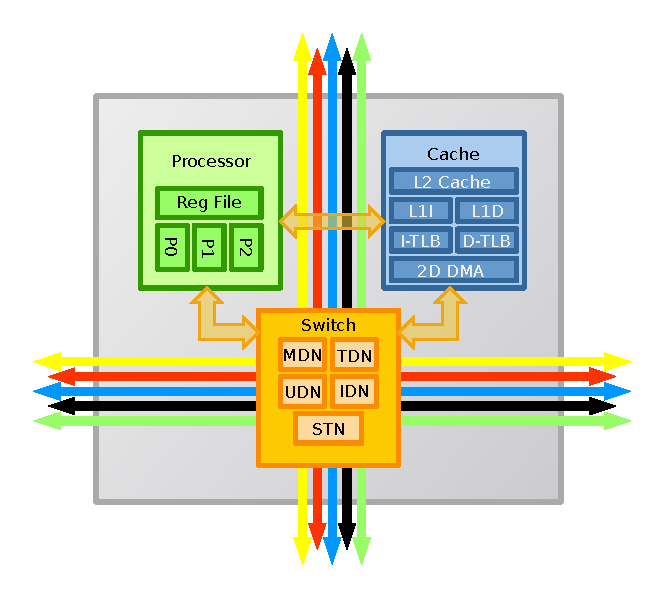
\includegraphics[width=0.5\textwidth]{images/tile64_cpu.pdf}
    \caption{TILEPro64 single processor diagram\cite{tilepro64-diagram}}
    \label{fig:tile64_cpu}
\end{figure}

Like seen in figure~\ref{fig:tile64_cpu}, every tile has three caches: L1D, L1I
and L2. L2 cache size is 64KiB. L3 is a "virtual cache" shared between tiles,
which size is 64KiB * 64 = 4MiB, thus creating 4 MiB of quickly accessible
on-chip cache.

\subsubsection{User Dynamic Network (UDN)}
Tilera has very interesting feature: User Dynamic Network, UDN. It is very low
latency (sending 130B message takes in the order of ticks) and high bandwidth
(order of tens of gigabits per second) switched inter-core network.

It can be very interestingly exploited in message-passing systems for
low-latency communication. Example of successful usage of this network is
presented in section~\ref{sec:future-work}.

\subsubsection{One or more Linux instances simultaneously}
TILEPro64 can run multiple Linux SMP instances on different tile configurations
(1-64 cores per Linux instance). In this project we run single Linux SMP
instance with 62 dedicated cores.

\subsubsection{Inter-core communication}
In current systems data exchange between cores is handled via shared memory,
while maintaining the coherency of the CPUs caches. Conversely, Tilera employed
a faster approach alongside: a high-bandwidth low-latency switched network
between the cores, which can be used by applications for very fast and low
latency data exchange directly between the CPUs\cite{tile64}.

From functional perspective, this kind of many-core system in many aspects
resembles a many-node cluster. Machines (tiles) communicate with each other by
sending messages; machines (tiles) can fail; they have to synchronize their
actions (think about locks and mutexes, which are much more complicated without
having shared memory). Since message-passing based many-core chips are coming to
the stage, it is important to investigate consensus algorithms in many-core
systems.

\subsection{Epiphany by Adapteva}

Adapteva is another many-core chip provider which aims to make many-core
computing cheap\cite{parallella-kickstarter}. From user's perspective
Adapteva's Epiphany\cite{epiphany} is similar to TilePRO64: it is a
network-on-chip, with many stand-alone cores, which can be used by userspace for
message sending between cores.  Figure~\ref{fig:epiphany_64} shows the block
diagram of Epiphany many-core chip.

\begin{figure}
    \centering
    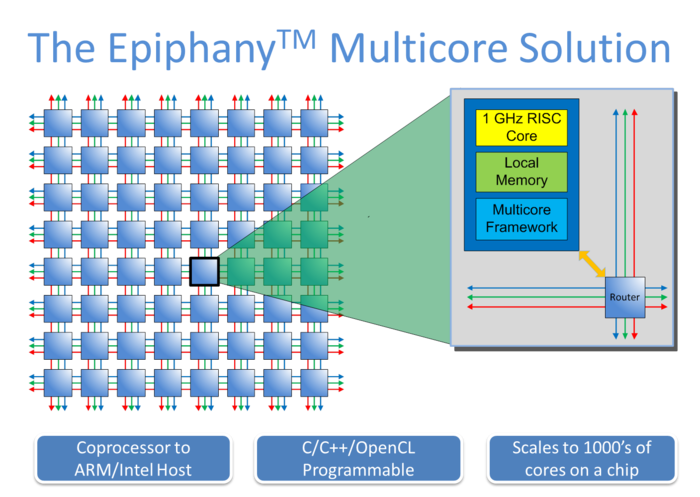
\includegraphics[width=0.5\textwidth]{images/parallella_64core.png}
    \caption{Adapteva's Epiphany\cite{parallella-kickstarter}}
    \label{fig:epiphany_64}
\end{figure}

Adapteva are estimating to deliver massively parallel chips in near future: a 1K
core chip by year 2014 and 16K core chip by year 2022.

\begin{figure}
    \centering
    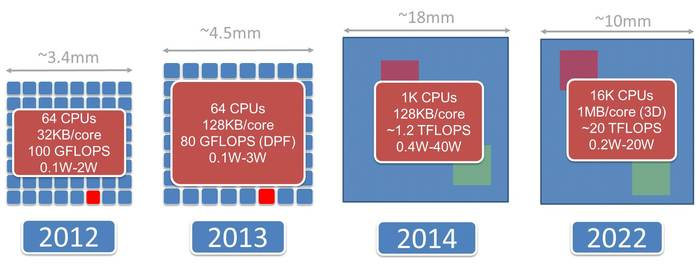
\includegraphics[width=0.5\textwidth]{images/parallella_future.jpg}
    \caption{Future of parallella\cite{parallella-kickstarter}}
    \label{fig:parallella_future}
\end{figure}

This proves that many-core NOC architectures are gaining popularity.

\section{Consensus and Paxos family overview}
\label{sec:paxos-family}

Paxos family algorithms are designed for reliably reaching a consensus in a
distributed system. The most primitive application is reliably learning a value
by a majority of acceptors. It works as follows: a set of proposers propose a
value, and the algorithm guarantees that only one value will be chosen by a
majority of acceptors. In worse case no value will be chosen.

The most popular application is distributed state machine implementation
\footnote{\url{http://en.wikipedia.org/wiki/Paxos\_(computer\_science)}}. A
majority of cluster nodes can use this algorithm to agree on an order in which
to execute a series of commands. A classical example for this is database
transaction synchronization across many database nodes, which have local copies
of data. State machine replication is built on the primitive of choosing a
single value.

Paxos algorithms are used primarily for synchronizing distributed systems. A few
notable examples: Google uses Paxos in their distributed locking service
Chubby\cite{chubby} (which is an important building block of BigTable). Another
example is OpenReplica\cite{openreplica}, where Paxos is used to implement a
replicated state machine.

\cite{paxos-simple} explains the classical way to implement a replicated state
machine:

\begin{quote}
To guarantee that all servers execute the same sequence of state machine
commands, we implement a sequence of separate instances of the Paxos consensus
algorithm, the value chosen by the $i^{th}$ instance being the $i^{th}$ state
machine command in the sequence.
\end{quote}

\subsection{Paxos as Black Box}

This section describes in high level what Paxos does. In the diagrams below
white ellipses are members of the cluster (machines or cores), rectangles are
proposed values, and the ellipse with "Paxos" is the Paxos black-box algorithm.

Scenario: a few nodes want to agree on some value. It can be an $i$'th command
in state machine, what's for lunch or some other value of interest that nodes
must agree on. Paxos will ensure that only one value will be learnt (in case of
failures, on value will be learnt, but then election can be retried after a
while).

Figure~\ref{fig:paxos-highlevel} shows a simplified flow of Paxos algorithm from
application developer's point of view. Note that that is almost all developer
needs to know about Paxos in order to be able to use epaxos\cite{epaxos}.

\begin{figure}
    \begin{subfigure}[b]{0.22\textwidth}
        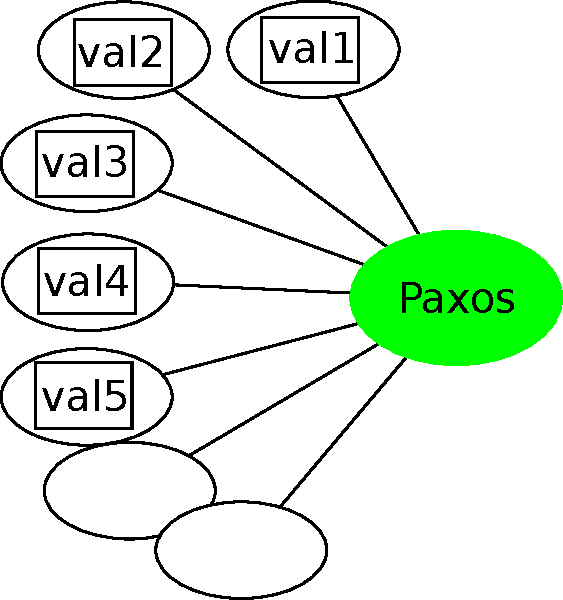
\includegraphics[width=\textwidth]{images/paxos1.pdf}
        \caption{Send values to Paxos "black box"}
    \end{subfigure}\hfill
    \begin{subfigure}[b]{0.32\textwidth}
        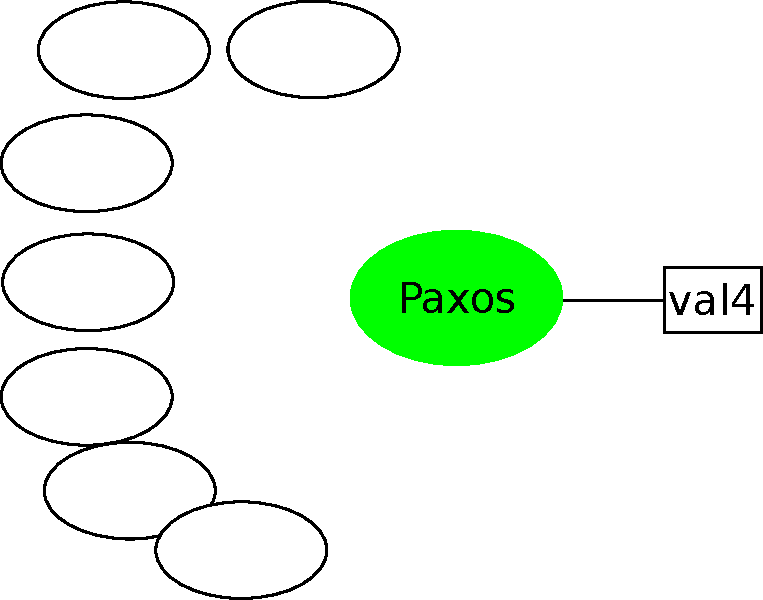
\includegraphics[width=\textwidth]{images/paxos2.pdf}
        \caption{val4 is elected}
    \end{subfigure}\hfill
    \begin{subfigure}[b]{0.32\textwidth}
        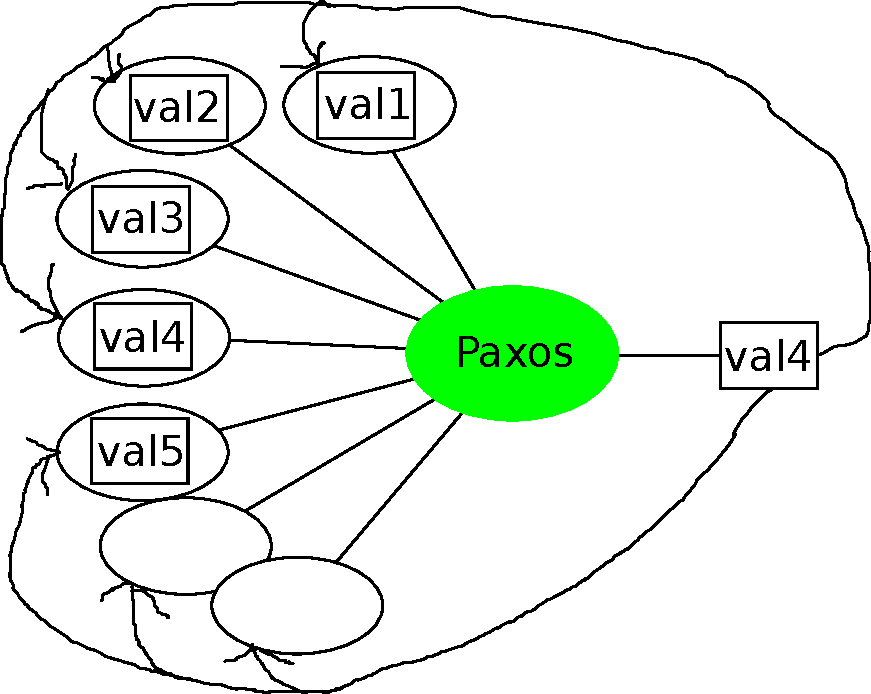
\includegraphics[width=\textwidth]{images/paxos3.pdf}
        \caption{val4 is broadcasted back and learnt}
    \end{subfigure}

    \caption{Paxos in high level}
    \label{fig:paxos-highlevel}
\end{figure}

Original Paxos algorithm is presented in \cite{classic-paxos} and
\cite{paxos-simple} by Leslie Lamport.

\subsection{About Paxos on many-core}

\subsubsection{Number of messages per election}

In a few places the exact behaviour of Paxos algorithm is left unspecified. For
example, a proposer must send its proposal to a {\em majority of acceptors}. If
there are 999 acceptors, the algorithm will be satisfied if the proposal will be
sent to 500, 750 or all 999 acceptors. In case there are no failures, sending
500 messages gives equivalent result as to sending 999 messages. It is up to the
developer to decide what is more important: safety or performance, or somewhere
in the middle.

Important property to know when designing a distributed system is how
communication volume increases with increasing number of participants. In Paxos
case, number of messages and number of participants are linearly correlated.
Also message size with increasing system is a concern. Because Paxos does not
store any participant information in the messages, message size does not
increase if the number of voters increases.

\subsubsection{Possible optimization using shared memory}

Paxos was designed for shared-nothing message-passing unreliable systems. That
means whenever a message about proposed value is sent, payload (the value
proposed) is always sent together. This is inefficient, because the value might
be sent only once to the learners, instead of going
proposer-acceptor-proposer-acceptor loop. On many-core systems with shared
memory this can be optimized by sending a reference to the proposed message
payload (or pointer in memory) instead of always sending the payload. The
learner can retrieve the payload from proposer when the election is over.

\section{Language Choice}
\label{sec:erlang-why}

The language decision was based on these factors:
\begin{enumerate}
    \item It can run on Tilera64.
    \item How well is it suitable for parallel algorithm implementation.
    \item Performance.
\end{enumerate}

\subsection{Cloud Haskell}

Initially Cloud Haskell\cite{cloud-haskell}  was chosen for the algorithm
implementation, for the following reasons. It is very convenient to program
state machines in a functional language; it compiles to machine code, which
makes it a good candidate for performance. Furthermore, llvm
backend\cite{llvm-haskell} looked like a promising sign for portability.

\begin{quote}
    Cloud Haskell is a library for distributed concurrency in Haskell. The
    purpose is to make it easier to write programs for clusters of machines. It
    provides a message passing communication model, inspired by and very similar
    to that of
    Erlang.\footnote{\url{http://www.haskell.org/haskellwiki/Cloud\_Haskell}}
\end{quote}

However, after some research it turned out that cross-compilation is impossible,
and the whole GHC must be ported to Tilera platform. Porting GHC to Tilera was
out of the scope of the project, so other languages were considered.

\subsection{Erlang}

Another language candidate was Erlang. Erlang is a general-purpose, concurrent,
and functional programming language developed by engineers from Ericsson in
1980s. Erlang is a language based on the  {\em actor model}, characterized by
the following features:

{\em Concurrency:} Erlang has extremely lightweight processes whose memory
requirements can vary dynamically. Processes have no shared
memory\footnote{They do in some circumstances for efficiency reasons, but this
is completely transparent to the programmer} and communicate by asynchronous
message passing.

{\em Distribution:} Erlang is designed to be run in a distributed
environment: it is as easy to create a process and communicate to
it on a host node like on a remote node.

The most appealing feature of Erlang is its approach to concurrency. Erlang {\em
actors} and message passing are higher-level synchronization primitives than
mutexes and condition variables. User can spawn millions of processes in Erlang
VM and Erlang will do a very good job in parallelizing their work with extremely
low context-switching and message passing overhead.

Erlang is written in C and requires standard UNIX tools to (cross-)compile and
run it. Supported platforms includes any Unix system, vxworks, Linux and
Windows
\footnote{\url{http://www.erlang.org/doc/installation\_guide/INSTALL.html}}.
Older version of Erlang (R13B) has been cross-compiled and ran on Tilera
Multi-core Development Environment (MDE) version 2. Some patches to the build
system were necessary to compile newer version of Erlang (R15B02) on the
version 3 of Tilera MDE. They have been submitted upstream.

\subsection{About Erlang Run Time System (ERTS)}

Under the hood Erlang virtual machine is a bytecode interpreter\footnote{for x86
systems there is an optional native code compiler \emph{hipe}\cite{hipe}, which
aims to improve computational performance}. Erlang itself is an OS process,
which main building parts are {\em schedulers} and {\em processes}. Erlang
processes are light-weight (grow and shrink dynamically) with small memory
footprint, fast to create and terminate and the scheduling overhead is low.
These are scheduled by Erlang run-time system. {\em Scheduler} is an OS thread
which schedules the Erlang processes. By default Erlang creates as many
schedulers as there are cores available. On Linux Erlang uses information about
CPU topology to exploit data locality.

An Erlang {\em node} is an Erlang VM instance which can talk to other nodes.
Several nodes can be on different machines. Nodes can communicate over TCP, SSL
and unix pipes (default and most popular is TCP). Processes within a node can
transparently send messages to other processes (semantics are the same as if
they were sent from the same node), monitor other nodes or processes. That all
means that in Erlang you can create a homogeneous cluster of nodes and speak to
the processes in other nodes using the same semantics as if the processes were
local (in the same node).

\section{Erlang evaluation on Tilera64}
\label{sec:erlang-eval}

\subsection{Related work}

A good example of a very robust synchronization between cores implementation
using message passing is memcached port to Tilera done by Facebook. UDN was used
for action orchestration and state synchornization\cite{facebook-tilera}. That
exhibited impressive performance compared to standard architecture servers.

Interest in suitability of software development with Erlang on multi-core
processors is increasing. For instance, Convey et~al.\cite{erlang-acoustic}
investigate the relative merits of C++ and Erlang in the implementation of a
parallel acoustic ray tracing algorithm. Marr et~al.\cite{vm-manycore} analyze
virtual machine support for many-core architectures including Erlang.

Jianrong \cite{erlang-manycore-scalability} analyzes performance characteristics
of Erlang virtual machine on Tilera64. The paper focused on benchmarking
\emph{embarrassingly parallel} programs (ones that can run without a need for
synchronization with each other). It achieved speedups of 30-40 by using 64
cores.

Project UPMARC\footnote{\url{http://www.it.uu.se/research/upmarc}} creates tools
that improve testing of many-core systems development. Number of them are
implemented in/for
Erlang/OTP
\footnote{\url{http://www.it.uu.se/research/upmarc/publications/researchers}}.

\begin{quote}
UPMARC's goal is to develop the insights that enable new tools and approaches to
make parallel programming easier, and to demonstrate their effectiveness through
prototype implementations on real problems.
\end{quote}

\begin{quote}
RELEASE\footnote{\url{http://www.release-project.eu/}} is an EU FP7 STREP
(287510) project that aims to scale the radical concurrency-oriented programming
paradigm to build reliable general-purpose software, such as server-based
systems, on massively parallel machines. The trend-setting language we will use
is Erlang/OTP which has concurrency and robustness designed in. Currently
Erlang/OTP has inherently scalable computation and reliability models, but in
practice scalability is constrained by aspects of the language and virtual
machine. Moreover existing profiling and debugging tools don't scale.
\end{quote}

\subsection{Erlang parallelism performance on TILEPro64}

Performance of Erlang on TILEPro64 with a program that does no synchronization
between the workers was tested. It works as follows: $Master$ process generates
$N$ lists with 100000 random numbers (where $N$ is number of workers) and spawns
a new $Worker$ process passing the generated list. Once all workers are spawned,
$Master$ sends a message to all the workers to {\tt begin work}. When $Master$
process receives a number from every worker, the program terminates.

$Worker$ process: it receives {\tt begin work} message, sorts the list and
sends median to the $Master$. Then terminates. Pseudocode:

\begin{algorithm}
    \begin{algorithmic}
        \Function{Master}{}
            \State $PidList \gets []$
            \State $N \gets 128$
            \For{every $N$}
                \State $L \gets$ list of 100000 random numbers
            \EndFor
            \State $Pid \gets spawn(Worker, L)$
            \Comment{spawn $Worker$ process and pass $L$ to it}
            \State Append $Pid$ to $PidList$
            \State $StartTimestamp \gets now()$
            \Comment{Start measuring execution time}
            \For{$Worker$ in $PidList$}
                \State $Worker$ ! {\tt 'begin work'}
                \Comment{send {\tt 'begin work'} to $Worker$}
            \EndFor
            \For{$Worker$ in $PidList$}
                \State receive $\_Number$
                \Comment{receive $\_Number$ (which is a median of some list) and
                discard it}
            \EndFor
            \State print $Delta \gets now() - StartTimestamp$
        \EndFunction

        \Function{Worker}{$L$}
            \Comment{note that worker receives $L$ on startup (big list)}
            \State receive {\tt 'begin work'}
            \Comment{wait until {\tt 'begin work'} is received from master}
            \State $L2 \gets sort(L)$
            \State $Master$ ! $median(L2)$
            \Comment{send median of $L2$ to $Master$}
        \EndFunction
        \Comment{at this point $Worker$ process terminates}
    \end{algorithmic}
    \caption{pseudo-code of embarrassingly parallel program}
    \label{alg:embarrassing}
\end{algorithm}

\subsubsection{Serial component in embarrassingly parallel program}

Note that this program actually has a serial component it's the sending messages
{\tt begin work} and gathering the median to the single process. To check the
real cost of it, a similar program was created to check just process spawning
and message sending overhead. It works the same way like
program~\ref{alg:embarrassing}, but instead of passing a list and an item, {\tt
ok} is passed to process and back. Master process creates 100000 workers, sends
each of them its {\em pid} and waits for 100000 {\tt ok}'s. Worker process
replies to the {\em pid} it received with an {\tt ok}.

On Intel Core Duo CPU @ 1.66GHz the whole process takes 0.85-0.9 seconds, or up
to $9\mu s$ per process. So the serial overhead of program~\ref{alg:embarrassing}
is not more than $9*256 = 2304 \mu s$, or no more than two and a half
milliseconds. With 1 core program\ref{alg:embarrassing} runs for around 5
minutes, so 2.5 milliseconds of serial component is overwhelmed by actual work
of the workers and can be neglected.

\subsection{Embarrassingly parallel program scalability and VM tuning}

We would expect this program to scale linearly while increasing number of cores.
Initial results of the benchmarks are shown in figure~\ref{fig:bad_speedup}.
The maximum speedup is around 12 with a spike to 14, and the results are very
unstable when increasing the number of cores. To summarize, initial benchmarks
show that Erlang VM without tuning on a many-core machine performs poorly.

\begin{figure}
    \centering
    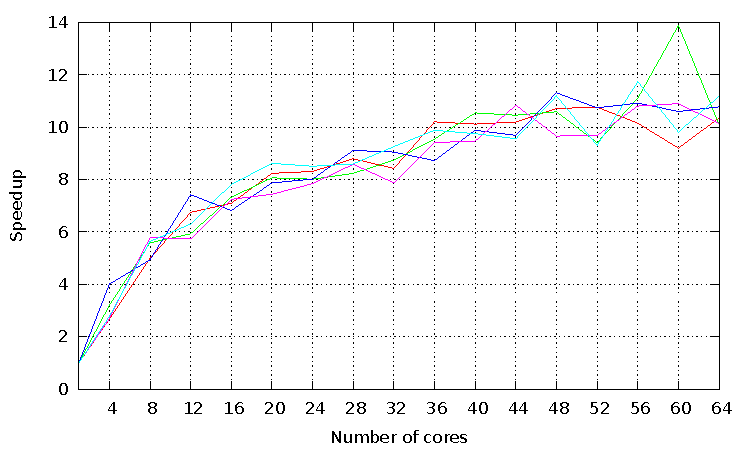
\includegraphics[width=0.9\textwidth]{images/bad_speedup.pdf}
    \caption{Initial speedup of algorithm~\ref{alg:embarrassing} (5 measurements)}
    \label{fig:bad_speedup}
\end{figure}

Kenneth Lundin gave a talk in Erlang Factory\cite{lundin-smp} about Erlang
many-core performance and suggested to pin Erlang schedulers (OS threads) to
hardware cores. This can be achieved by passing {\tt +sbt db} flag on during
startup of the Erlang virtual machine. This adjustment gave significant
improvement: performance stabilized and jumped to around 37 for 56 cores, as
shown in figure~\ref{fig:parallel_speedup}.

\begin{figure}
    \centering
    \includegraphics[width=0.9\textwidth]{images/speedup.pdf}
    \caption{Speedup of algorithm~\ref{alg:embarrassing}}
    \label{fig:parallel_speedup}
\end{figure}

\begin{figure}
    \centering
    \includegraphics[width=0.9\textwidth]{images/slowdown.pdf}
    \caption{Slowdown of algorithm~\ref{alg:embarrassing} (derived
    from figure~\ref{fig:parallel_speedup})}
    \label{fig:parallel_slowdown}
\end{figure}

Figure~\ref{fig:parallel_slowdown} is derived from~\ref{fig:parallel_speedup}
and shows precisely the loss of speedup while increasing the number of cores.

This experimental data shows that Erlang scales pretty well with increasing
number of cores. More details about it can be found in work by
Jianrong\cite{erlang-manycore-scalability}.

Currently in Erlang message sending between processes is implemented using
shared memory, locks and mutexes. However, it would be a very interesting
project to replace inter-erlang-process communication with UDN thus eliminating
the shared memory. Most importantly, application developer would not notice the
usability change; however, this would potentially eliminate a lot of bottle-neck
during message passing which incurs by going out of chip.

\section{Clasic Paxos in Erlang}
\label{sec:paxos-api}

As of now I was able to find three Classic Paxos implementations in Erlang
\footnote{\url{https://github.com/gburd/gen\_paxos}}
\footnote{\url{http://libpaxos.sourceforge.net/paxos\_projects.php\#erlangpaxos}}
\footnote{\url{http://code.google.com/p/scalaris/}}, but they are written in a
way that it will be very difficult to extend the algorithm. Therefore classic
paxos has been reimplemented.

See appendix~\ref{sec:spec-syntax} for a quick syntax introduction to Erlang
{\tt -spec} syntax.

\begin{figure}
    \begin{verbatim}
    -type fsmref() :: reference().
    -type value() :: term().
    -type learner_callback() :: fun((value()) -> ok).

    %% Specify learner function per election.
    %% The passed function will be executed when a value is learned.
    -spec init_learner(fsmref(), learner_callback()) -> ok.

    %% Executed by application in order to propose a value
    -spec propose(fsmref(), value()) -> ok.
    \end{verbatim}
    \caption{API of Classic Paxos\cite{epaxos}}
    \label{fig:paxos-api}
\end{figure}

To propose a value, application calls {\tt propose()}. When the value (same or
other one) is learned, user's callback {\tt learn()} is called.

{\tt fsmref()} is an \emph{election} and \emph{electorate} identifier. It is
acquired during the start-up of proposers, acceptors and learners; in this work
we are not concerned about the start-up of the cluster and how this value is
generated.

\section{Conclusion}
\label{sec:conclusion}

Erlang programming language is suitable for algorithm implementation on
many-core systems.

\subsection{Future work}
\label{sec:future-work}

Using UDN for message passing in Erlang virtual machine would also be a very
interesting project. Moreover, the implementation of
Paxos\footnote{\url{https://github.com/Motiejus/epaxos}} is planned to be used
in industrial environment in a cluster management application.

\subsection{Acknowledgement}

The author thanks Wim Vanderbauwhede for his comments and continuous support in
all phases of this personal project.

\clearpage
\begin{thebibliography}{99}

    \bibitem{hipe} Sagonas,~K., Wilhelmsson,~J. \emph{Efficient memory
        management for concurrent programs that use message passing}. Science of
        Computer Programming, 62(2): p.~98-121, October 2006.

    \bibitem{1kcorechips} Borkar,~S. \emph{Thousand Core Chips—A Technology
        Perspective}. DAC '07 Proceedings of the 44th annual Design Automation
        Conference. p.~746-749.

    \bibitem{pollack} Pollack,~F. \emph{Pollack's Rule of Thumb for
        Microprocessor Performance and Area.}

    \bibitem{future-microprocessors} Borkar~S., Chien,~ A.~A. \emph{The Future
        of Microprocessors}. Communications of the ACM, Vol. 54 No. 5, p.~67-77.

    \bibitem{tile64} Bell,~S., Edwards,~B., Amann,~J., Conlin,~R.,
        Joyce,~K., Leung,~V., MacKay,~J., Reif,~M., Bao,~L., Brown,~J.,
        Mattina,~M., Miao,~Chyi-Chang, Ramey,~C., Wentzlaff,~D.,
        Anderson,~W., Berger,~E., Fairbanks,~N., Khan,~D., Montenegro,~F.,
        Stickney,~J., Zook,~J. \emph{TILE64 -- Processor: A 64-Core SoC with
        Mesh Interconnect}. Solid-State Circuits Conference, 2008. ISSCC 2008.
        Digest of Technical Papers. IEEE International. p.~88-598.

    \bibitem{classic-paxos} Lamport,~L. \emph{The part-time parliament}. ACM
        Transactions on Computer Systems (TOCS). Volume 16 Issue 2, May~1998.
        p.~133-169.

    \bibitem{paxos-simple} Lamport.,~L. \emph{Paxos made simple}. ACM SIGACT
        News (Distributed Computing Column) 32, 4 (Whole Number 121, December
        2001) p.~51-58.

    \bibitem{generalized-consensus} Lamport.~L. \emph{Generalized Consensus and
        Paxos}. Microsoft Research Technical Report MSR-TR-2005-33.

    \bibitem{chubby} Burrows,~M. \emph{The Chubby lock service for
        loosely-coupled distributed systems}. OSDI '06 Proceedings of the 7th
        symposium on Operating systems design and implementation. p. 335-350.

    \bibitem{openreplica} Altinbuken,~D., Emin~Gun.,~S. \emph{Commodifying
        Replicated State Machines with OpenReplica}. Computing and
        Information Science Technical Reports, Cornell University.

    \bibitem{erlang-acoustic} Convey,~C., Fredricks,~A., Gagner,~C.,
        Maxwell,~D., Hamel,~L. \emph{Experience report: erlang in acoustic ray
        tracing}. In ICFP ’08: Proceeding of the 13th ACM SIGPLAN international
        conference on Functional programming, pages 115–118, New York, NY, USA,
        2008. ACM.

    \bibitem{vm-manycore} Marr,~S. D’Hondt,~T. \emph{Many-core virtual machines:
        decoupling abstract from concrete concurrency}. In SPLASH ’10:
        Proceedings of the ACM international conference companion on Object
        oriented programming systems languages and applications companion.
        p.~239–240, New York, NY, USA, 2010. ACM.

    \bibitem{erlang-manycore-scalability} Jianrong, Z. \emph{Characterizing the
        Scalability of Erlang VM on Many-core Processors}. Student thesis, KTH,
        School of Information and Communication Technology (ICT).

    \bibitem{facebook-tilera} Berezeckia,~M., Frachtenberga,~E. Palecznya,~M.
        Steeleb,~K. \emph{Power and performance evaluation of Memcached on the
        TILEPro64 architecture}. Sustainable Computing: Informatics and Systems.
        Volume 2, Issue 2, June 2012, p. 81–90.

    \bibitem{amdahls-law} Hill,~Mark~D. \emph{Amdahl's Law in the Multicore
        Era}. Dept. of Comput. Sci., Univ. of Wisconsin-Madison, Madison, WI
        Marty, Michael R.  Vol.~41, Issue~7. p.~33-38.

    \bibitem{lundin-smp} Lundin,~K. \emph{About Erlang/OTP and Multi-core
        performance in particular}. Talk at Erlang Factory London June 26 2009.

    \bibitem{epiphany} Adapteva. \emph{Adapteva Epiphany multi core
    architecture}.

    \bibitem{parallella-kickstarter} Adapteva. \emph{Parallella - a
    supercomputer for everyone}. {\small \url{
http://kickstarter.com/projects/adapteva/parallella-a-supercomputer-for-everyone
}}

    \bibitem{epaxos} Classic Paxos implementation in Erlang. {\small \url{
    https://github.com/Motiejus/epaxos}}.

    \bibitem{tilepro64-diagram} Agarwal,~A. \emph{Proceedings of HPEC Workshop,
    2007}.

    \bibitem{cloud-haskell} Peyton-Jones,~S. \emph{Towards Haskell in the
    cloud}. Proceedings of the 4th ACM symposium on Haskell. p.~118-129.

    \bibitem{llvm-haskell} Terei,~D.~A., Chakravarty,~M.~T.~M. \emph{An llVM
    backend for GHC}. Proceedings of the 3rd ACM Haskell symposium on Haskell
    p.~109-120.

\end{thebibliography}

\begin{appendices}

\section{Erlang type specification syntax}
\label{sec:spec-syntax}

This is a quick tutorial to Erlang type specification syntax, which should be
enough to understand Paxos API in section~\ref{sec:paxos-api}. Examples of
equivalent type definitions in Haskell are provided. Haskell knowledge to
understand this section is useful, but not mandatory.

A few important differences in the type systems: type names in Erlang must be
lowercase, whereas in Haskell they must be uppercase. Another difference is that
Erlang functions to dot support currying. Erlang functions are uniquely defined
by Name/Arity pair, where Arity is the number of arguments the function accepts.

\subsection{Value definitions}

Erlang has a few primitive types: {\tt fun()}, {\tt integer()}, {\tt bool()},
etc. A composite type (or type alias if the type is simple) in
figure~\ref{fig:erlang-simple-type}.

\begin{figure}
    \begin{verbatim}
-type kv() :: {string(), integer()}.
-type map() :: [kv()].
    \end{verbatim}
    \caption{Simple Erlang type definition}
    \label{fig:erlang-simple-type}
\end{figure}

{\tt kv()} is a 2-tuple with first element {\tt string()} and second element
{\tt integer()}. Subsequently {\tt map()} is a list of {\tt kv()}s, which makes
it a simple map. It is equivalent to a definition in Haskell in
figure~\ref{fig:haskell-simple-type}.

\begin{figure}
    \begin{verbatim}
Kv :: (String, Integer)
Map :: [Kv]
\end{verbatim}
    \caption{Equivalent Haskell definition}
    \label{fig:haskell-simple-type}
\end{figure}

Both Haskell and Erlang example can be simplified to a single definition,
figure~\ref{fig:haskell-erlang}.

\begin{figure}
    \begin{verbatim}
-type map() :: [{string(), integer()}]. %  erlang
Map :: [(String, Integer)]              -- haskell
    \end{verbatim}
    \caption{Erlang and Haskell together}
    \label{fig:haskell-erlang}
\end{figure}

\subsection{Function type definitions}

Since functions are first-class data types in Erlang, rich type language exists
to specify their signatures. It is similar to previous example, but function
definition is a "special" type {\tt fun()}, figure~\ref{fig:fun}. This example
types a function which takes integer as one argument and returns a boolean.

\begin{figure}
    \begin{subfigure}[b]{\textwidth}
        {\small \begin{verbatim}
-type filter_fun() :: fun((integer()) -> bool()).
            \end{verbatim}
        }
        \caption{Erlang}
    \end{subfigure}

    \begin{subfigure}[b]{\textwidth}
        {\small \begin{verbatim}
FilterFun :: Integer -> Bool
            \end{verbatim}
        }
        \caption{Haskell}
    \end{subfigure}
    \caption{Simple function type definition}
    \label{fig:fun}
\end{figure}


\subsection{Function signature definitions}

There is special syntax for defining function signatures, the {\tt -spec}
keyword. Example in figure~\ref{fig:spec}.

\begin{figure}
    \begin{subfigure}[b]{\textwidth}
        \begin{verbatim}
-spec cmp(integer(), integer()) -> lt | eq | gt.
        \end{verbatim}
        \caption{Erlang}
    \end{subfigure}

    \begin{subfigure}[b]{\textwidth}
        \begin{verbatim}
cmp :: Integer -> Integer -> LT | EQ | GT
        \end{verbatim}
        \caption{Haskell}
    \end{subfigure}
    \caption{Function signature}
    \label{fig:spec}
\end{figure}

\end{appendices}

\clearpage

\educationalconsent

\end{document}
